% !TEX root = ../thesis_main.tex

\section{Replicating Rockstuhl et al 2005} \label{chap:rep_rockstuhl}
\graphicspath{{replication_validation/figs/}}

When looking for results to attempt the validation of \pygbe we found the study of Rockstuhl et al. 2005 \cite{rockstuhl2005}. 
Even though their work consist on simulations and therefore does not qualify for a validation study, we decided to 
attempt the replication of one of their results. 

Rockstuhl and coworkers, in their paper "Analysis of the phonon-polariton response of silicon carbide microparticles 
and nanoparticles by use of the boundary element method", study the phonon-polariton response of silicon carbide (SiC)
nanoparticles using boundary element method. They use a two dimensional model developed previously on their group \cite{rockstuhl2003}
to analyze 6H-SiC multiple "cylindrical particles" (third dimension tends to infinity). The results presented on Figure 14 of their paper  
present the scattering cross-section of a SiC rectangular cylinder for different aspect ratios, and the case with $a = 672$ nm and $b = 328$ nm
was a perfect candidate given that these dimensions comply with our quasistatic approach.

In the work of Rockstuhl et al., they compute scattering cross section while with \pygbe we compute the extinction cross-section 
(absorption plus scattering). In the quasistatic regime absorption dominates over scattering, therefore these results are not directly
comparable. However, when having materials which show narrow and sharp peaks on their spectra, the wavelength at which the peaks occur 
in the scattering and extinction spectra, are nearly the same. For example, in the work of Wiley et al. \cite{wiley-etal-2006}
we see that for a silver nanocube, the wavelength at which the main peaks occur for extinction and scattering, are nearly the same. Due to the properties 
of silicon carbide, its spectra presents sharper and narrower peaks than silver, which leads to closely aligned extinction and scattering peaks.


\textbf{Differences in method and input data}

\begin{itemize}

\item {The main difference between the simulations in Rockstuhl and the ones performed with \pygbe is that the original results where obtained 
using a 2D boundary element method that solves full Maxwell equations, while we solve a 3D problem with the quasistatic limit approximation.}

\item{ Rockstuhl et al. work did not have a section with details on their simulations such as discretization of the geometries or parameters 
involved in their simulations. We chose parameters for our solver based on our previous experiences, and for the discretization of our 
geometries we performed a grid-independence study to ensure that we are minimizing discretization errors. It is worth noting that Rockstuhl
et al. geometries consist in two dimensions (infinite third dimension), while we perform the computations using a full 3D representation of the geometry.} 

\item {Regarding the complex dielectric constant, the study we aim to replicate uses 6h-SiC and their data comes from a source that we were not able
to replicate. As a replacement, we are using experimental data of 4H-SiC provided to us by the authors of Ellis et al. \cite{ellis2016} via 
private communications.}

\end{itemize}

\subsection{Grid independence study} \label{ssec:grid_indep_rock}

The equations that we solve in this problem are the same as the ones we solved in chapter \ref{sec:pot_elec_field} where we show grid convergence for the case of 
a silver sphere. In the work of Rockstuhl et al. \cite{rockstuhl2005} the geometries are cubes and prisms, and due to the nature of the geometries 
and their sharp edges, it was hard to find a case where we could see proper convergence using richardson extrapolation. Since we have show convergence for this type of physics
for the case of the sphere and given the difficulty of the sharp edges, we decided to settle with a grid-independence study. We performed the grid-independence study
on a similar setup to the case ib Fig. 18 of Rockstuhl et al. \cite{rockstuhl2005}, a cube of side $L=535$ nm surrounded by air, under a constant electric field aligned with the 
z-axis. Figure \ref{fig:cube535} shows the grid-independence study where we use a mesh with 15,552 triangles and a 19,200 triangles 
(from 9.05 $\times$ 10$^{-5}$ to 1.11 $\times$ 10$^{-4}$ triangles per $\text{\AA}$ squared) and the computed results are indistinguishable from each other.
We want to remark that the spectrum presented in Figure \ref{fig:cube535} has an extra peak compared to the one presented in Fig. 18 of Rockstuhl et al. \cite{rockstuhl2005}. We attribute
this extra peak to the three-dimensional nature of the geometry used in our model and the sharp edges, the latter effect also being mentioned by the Rockstuhl et al.
In the following sections we will present the replication study of one of the results on Figure 14 of Rockstuhl et al. and we will the effects of the 3D model as well as the sharpness of the edges. 

\begin{figure}
    \centering
    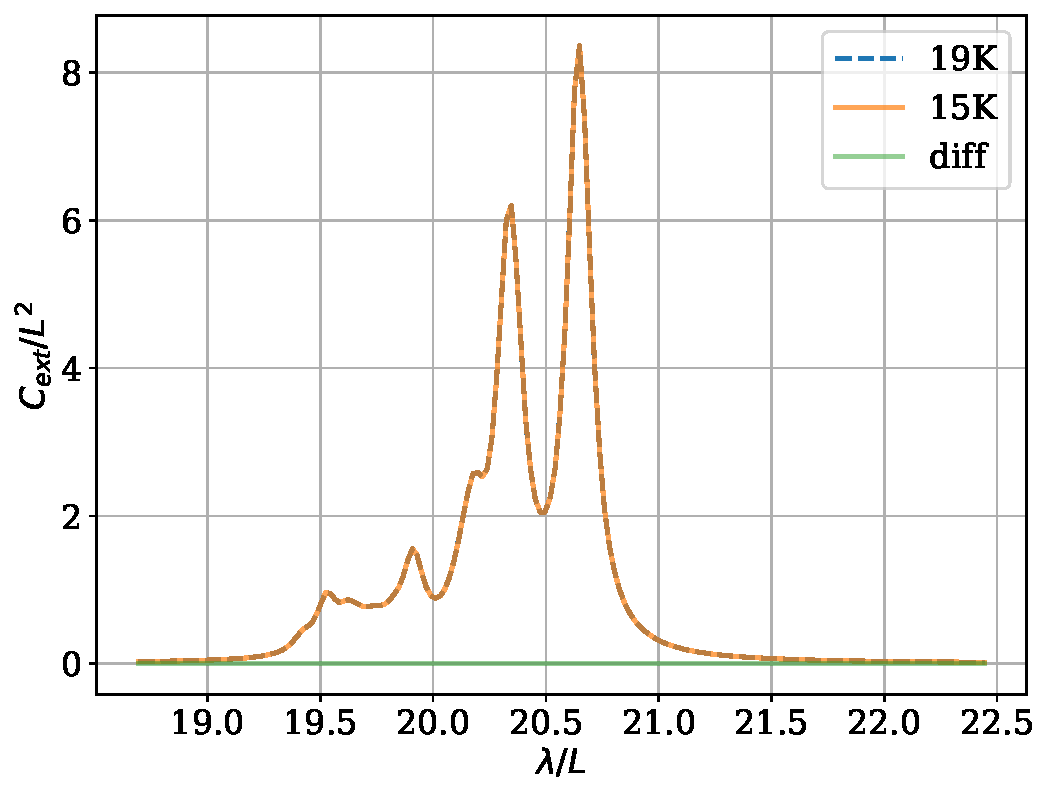
\includegraphics[width=0.75\textwidth]{cubeL535nm_15Kvs19K.pdf} 
    \caption{Grid-independence study for a SiC cube of side $L=535$ nm submerged in air under a constant 
    electric field in the $z$-direction. The curves represent the extinction cross-section divided by $L^2$ 
    as a function of wavelength divided by $L$, for mesh sizes 19K = 19,200 triangles and 15K = 15,552 triangles. 
    The label "diff" refers to the difference between the results of the two meshes.}
    \label{fig:cube535}
 \end{figure}

 \subsection{Replication of Figure 14 (case a1) of Rockstuhl et al., 2005}

 We chose to replicate the case "a1" ($a=672$ nm and $b=328$ nm) from the Figure 14 from Rockstuhl et al., 
 this case has dimensions that are within the quasistatic limit used in \pygbe. Rockstuhl and coworkers show the normalized
 scattering cross-section of a SiC rectangular cylinder, and they perform simulations for the setups showed in the Figure
 \ref{fig:rectangle_sketch}. In Figure \ref{fig:rectangle_sketch} (A) the electric field is parallel to the long side of the geometry, which 
 corresponds to the configuration of Figure 14 (right) of Rockstuhl et al. where the wave vector (illumination) goes along the short side of the geometry. 
Similarly, we see that in Figure \ref{fig:rectangle_sketch} (B) the electric field is parallel to the short side of the geometry, which 
corresponds to the configuration of Figure 14 (left) of Rockstuhl et al. where the wave vector (illumination) goes along the long side of the geometry
For the mesh of the rectangular prisms we used densities like the ones used in the grid-independence study (section \ref{ssec:grid_indep_rock}) or finer. We needed to elongate
the third dimension to the point that it represented "infinity". Figure \ref{fig:ext_y_14} shows the results of extending the third dimension ($y$ axis) to 
$y=1344$ nm ($2\times a$) and $y=2688$ nm ($4\times a$). We can see that when $y$ takes the longer value, the intensity of some peaks decreases, due to their association to 
the y-component. We have not explored larger values of $y$ because are limited by the quasistatic limit.
 \begin{figure}
    \centering
    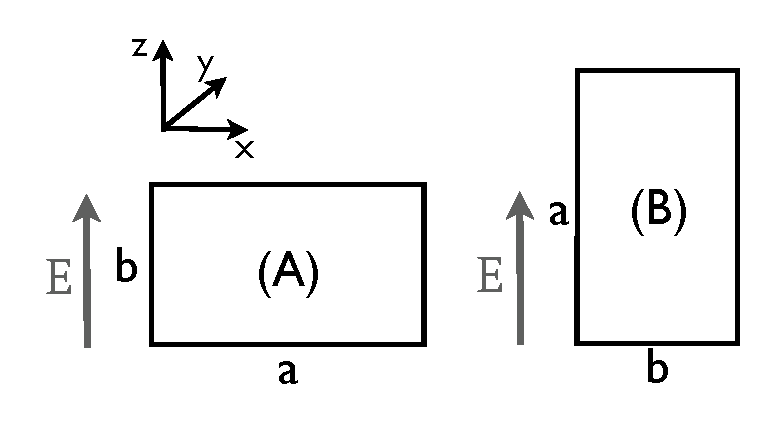
\includegraphics[width=0.45\textwidth]{rockstuhl_rectangles.pdf} 
    \caption{Configurations for the simulations corresponding to Fig. 14 of Rockstuhl et al., 2005.}
    \label{fig:rectangle_sketch}
\end{figure}

\begin{figure}
    \centering
    \subfloat{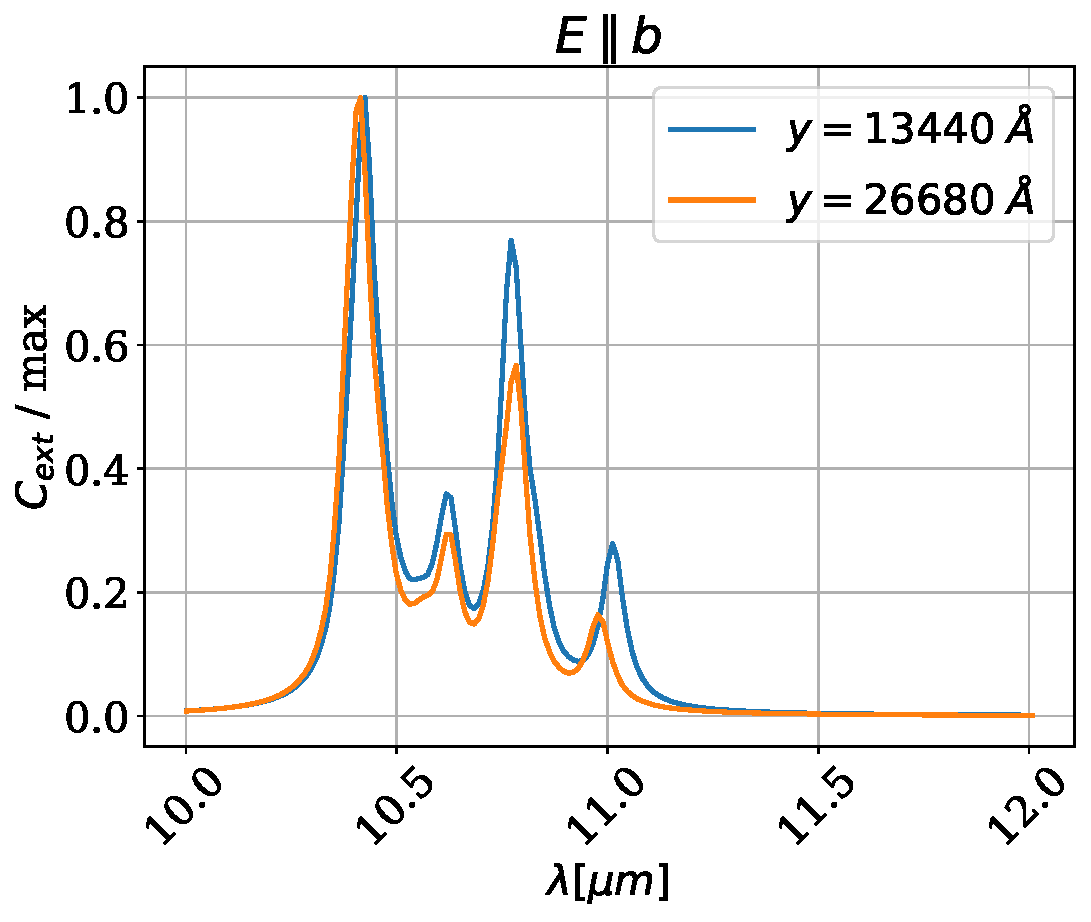
\includegraphics[width=0.48\textwidth]{ext_y_14a.pdf}}
    \subfloat{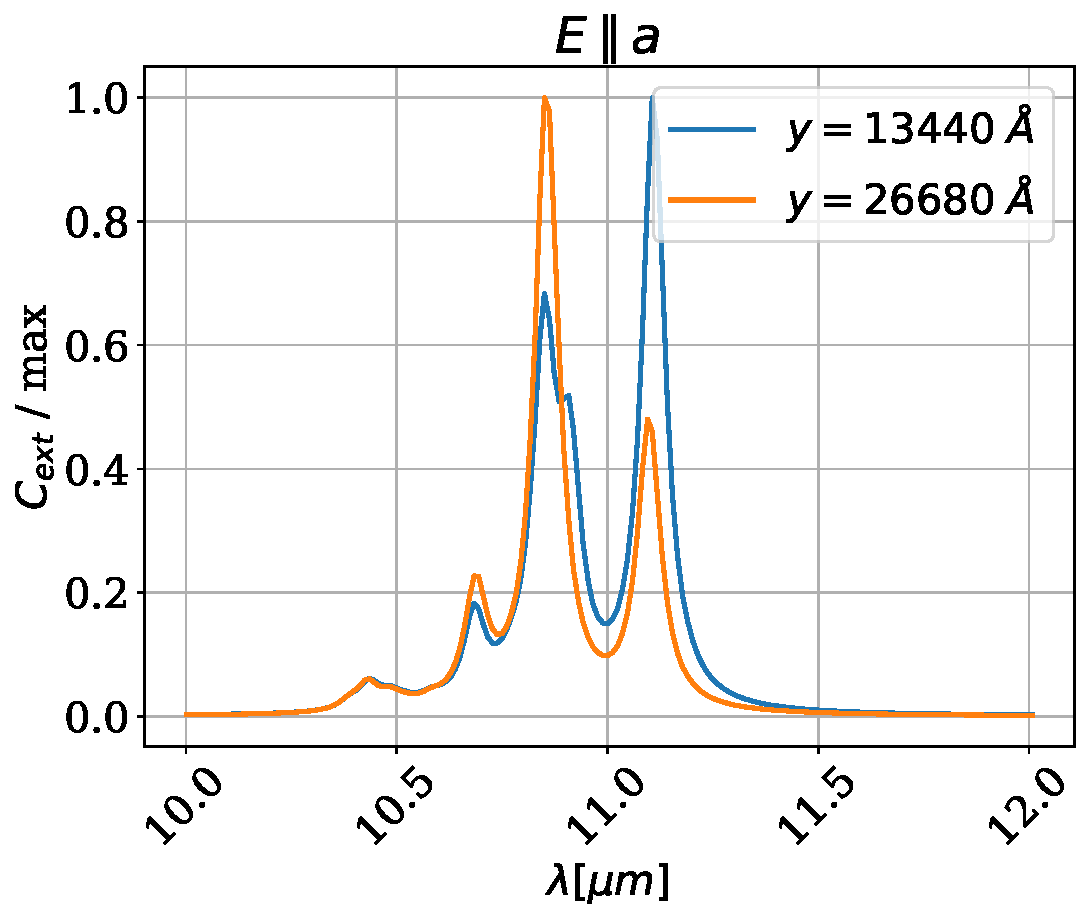
\includegraphics[width=0.48\textwidth]{ext_y_14b.pdf}} 
    \caption{Effect of the elongation of the third dimension ($y$) on the 
        extinction cross-section of a rectangular prism of SiC of dimensions $a=672$ nm 
        and $b=328$ nm, submerged in air and under a constant electric field 
        parallel to the $z$-axis. The left plot corresponds to a configuration such that the electric 
        field is parallel to $b$ (configuration (A) on Figure \ref{fig:rectangle_sketch}), while the 
        right plot corresponds to a configuration such that the electric field is 
        parallel to $a$ (configuration (B) on Figure \ref{fig:rectangle_sketch}.}
    \label{fig:ext_y_14}   
 \end{figure}

For the simulations of Figure \ref{fig:ext_y_14} we generated the meshes using an open source software Trimesh (\url{https://github.com/mikedh/trimesh}), 
but we realized that the mesher did not produce a uniform mesh and that it was not possible to obtained one with the functions available. To solve this problem 
we created a uniform mesh with our own Python script. We wanted to study the effect of using a uniform mesh and the roundness of the edges, the latter being mentioned by 
Rockstuhl et al. as a cause of the appearance of extra peaks. To generate the roundness of the geometries we relied on Trimesh (we give as input the uniform mesh generated 
with our Python script), however, we did not have control of the roundness as a function of the geometry dimensions or arc of curvature, so we used the default settings of
the software. Figure \ref{fig:tri_reg_round_14} shows the results of the effect of mesh uniformity and roundness of the edges of the geometry. We can see that in the for 
both orientation of the geometry ($E\parallel b$ and $E\parallel a$) the second peak located at $\approx$ 10.6 $\mu$m is much diminished in the green curve. These effects 
can be attributed to the roundness of the edges, what is consistent with the results of Rockstuhl et al. Once we have found the "best" meshed geometry (uniform mesh plus 
round edges) that we can construct, we can compare our results (green curve \ref{fig:tri_reg_round_14}) with the ones in Rockstuhl et al. Figure 14. We present the replication 
results in Figure \ref{fig:rep_14}, and we can see that the main resonance peaks in Figure 14 of Rockstuhl et al. are closely matched. We still have a third peak in our 
results, but we attribute this to the effects introduced by using a 3D geometry. We obtained the data from Rockstuhl's curves by using the WebPlotDigitizer
(\url{https://apps.automeris.io/wpd/}).
 

 \begin{figure}
    \centering
    \subfloat{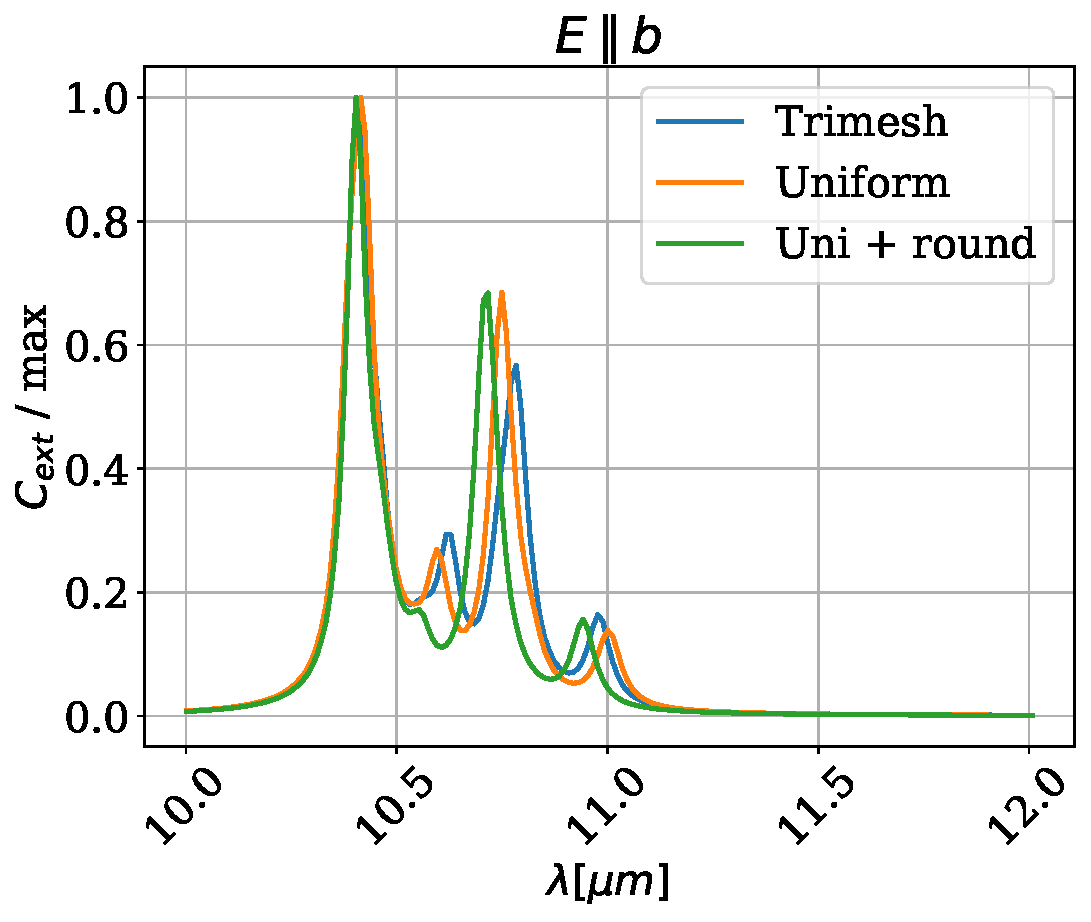
\includegraphics[width=0.48\textwidth]{tri_reg_round_14a.pdf}}
    \subfloat{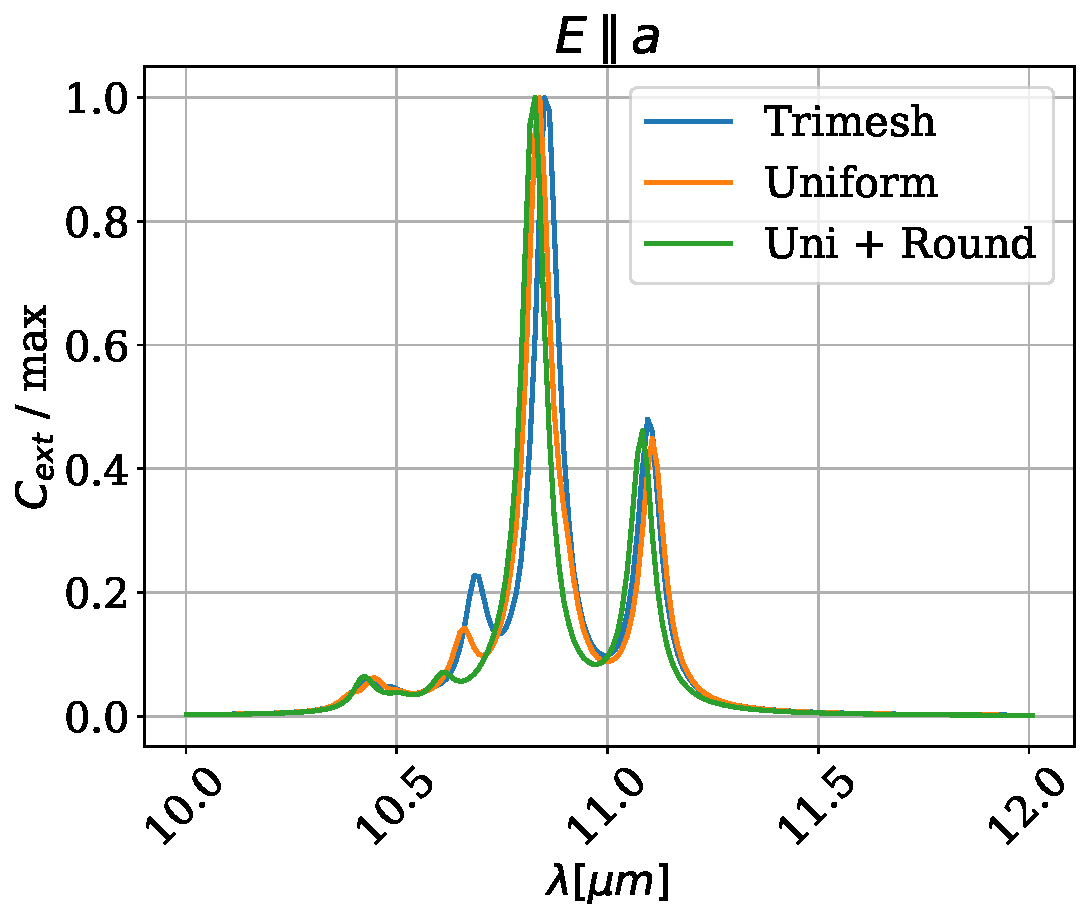
\includegraphics[width=0.48\textwidth]{tri_reg_round_14b.pdf}}
    \caption{Effect of uniformity of the mesh and roundness of the edges on the 
    extinction cross-section of a rectangular prism of SiC of dimensions $a=672$ nm, 
    $b=328$ nm and $y=2688$ nm, submerged in air and under a constant electric field 
    parallel to the $z$-axis. The labels are: \textbf{Trimesh}, for a non-uniform mesh generated using Trimesh; 
    \textbf{Uniform}, for a uniform mesh generated using Python scripts; and 
    \textbf{Uni + round}, for a uniform mesh generated using Python scripts with round 
    edges obtained using Trimesh.}
    \label{fig:tri_reg_round_14}
 \end{figure}

 \begin{figure}
    \centering
    \subfloat{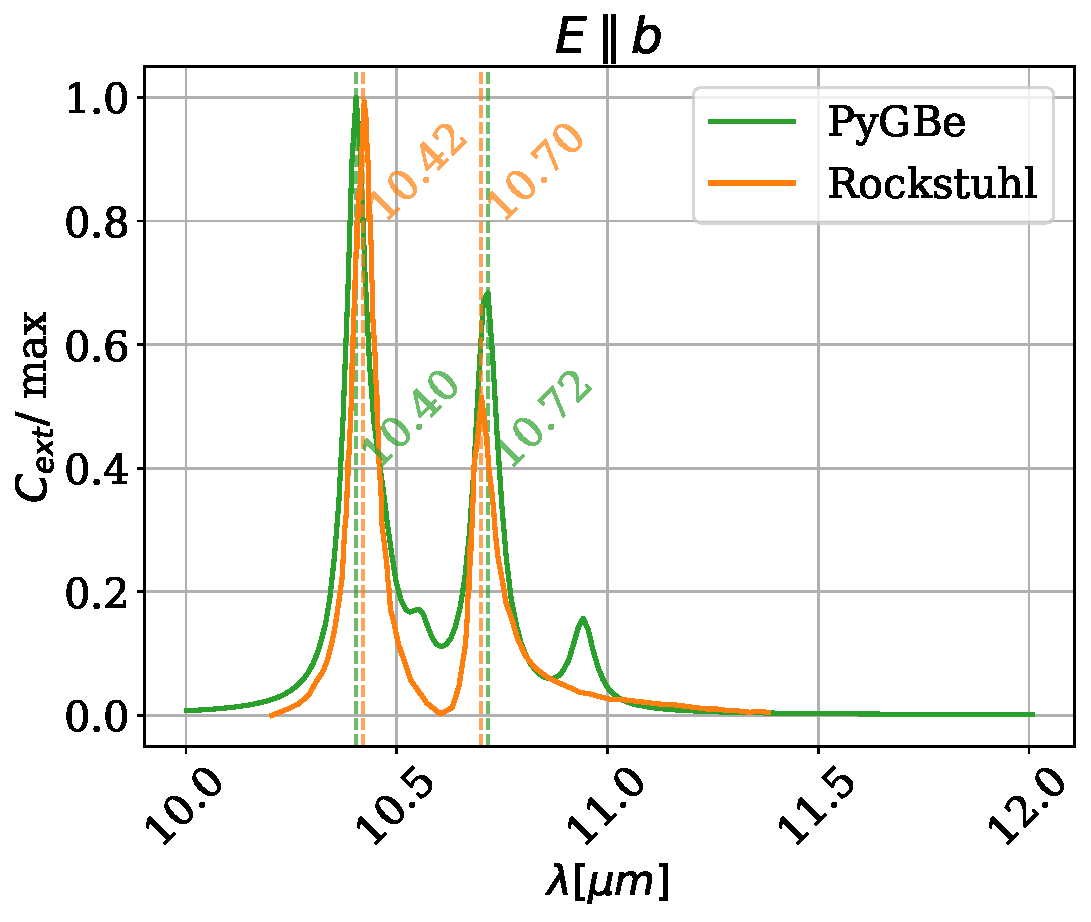
\includegraphics[width=0.48\textwidth]{replication_14a.pdf}}
    \subfloat{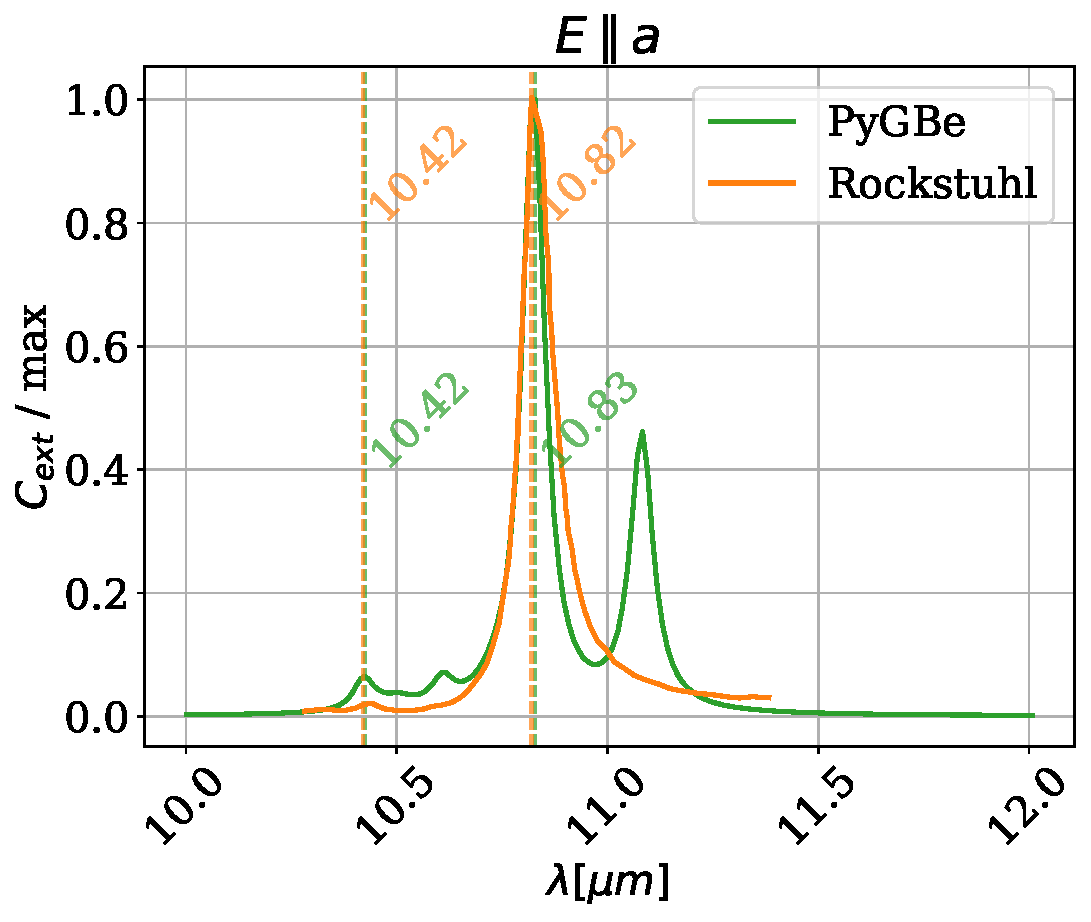
\includegraphics[width=0.48\textwidth]{replication_14b.pdf}} 
    \caption{Replication of the results in Figure 14 of Rockstuhl et al., 2005. Extinction cross-section of a
    rectangular prism of SiC of dimensions $a=672$ nm, $b=328$ nm and $y=2688$ nm, submerged
    in air and under a constant electric field parallel to the $z$-axis (green line). 
    The digitized curve from Rockstuhl et al.\ corresponds to scattering (orange line).}
    \label{fig:rep_14}
 \end{figure}

In this section we aim to replicate a result from Rockstuhl et al., 2005 \cite{rockstuhl2005} presented in Figure 14 of their paper. 
They computed the scattering cross-section as a function of wavelength for a silicon carbide rectangular cylinder, and reported the
numeric value of the resonance wavelengths in the text. They computed their results using a two-dimensional boundary element solver, 
but the data behind the plots was not available, so we manually digitize the values from the figure. In Figure \ref{fig:rep_14} we 
showed the comparison between our results and the digitized version of theirs. We succeed at replicating the peaks reported by 
Rockstuhl et al.\ at wavelengths 10.42 $\mu$m and 10.7 $\mu$m,  when the electric field $E$ is parallel to the short side of 
the rectangle, and 10.42 $\mu$m and 10.82 $\mu$m when $E$ is parallel to the long side. However, our results contain extra smaller peaks 
that are not present in Rockstuhl et al. The first one located between the main two peaks, which we attribute to the effect of sharp edges, 
since when we introduce roundness, it diminishes (see Figure \ref{fig:tri_reg_round_14}). The second extra peak, on the far right of the spectra, 
we attribute it to the 3D nature of the geometry, since the intensity of the peak decreases as the third dimension of the prism lengthens
(see Figure \ref{fig:ext_y_14}). As we mentioned before the quantity of interest in these findings is the wavelength at which the resonance peaks
occur, we can state that our results match and replicate the findings of Figure 14 of Rockstuhl et al. where $a = 672$ nm and $b = 328$ nm.
